\documentclass[11pt,a4paper]{report}
\usepackage{amsmath}
\usepackage{booktabs}
\usepackage{graphics}
\usepackage[dvipdfmx]{graphicx}
\usepackage{epsfig}
\DeclareGraphicsExtensions{.eps,.pdf,.jpg,.png}
\DeclareGraphicsRule{.jpg}{eps}{.bb}{}
\DeclareGraphicsRule{.png}{eps}{.bb}{}
\everymath{\displaystyle}
\setlength\parindent{0pt}
\begin{document}

\title{Lab3 Report}

\author{Ye Feiyang \and Cao Pozhi \and Yuan Xiaojie}

\date{Aug 10, 2012}

\maketitle

\section*{Introduction}
There are two widely used couplers, namely the Rat-Race coupler(180\(^o\) hybrid) and the Barnch-Line coupler(90\(^o\) hybrid).\\

For Rat-Race coupler, \\
\begin{equation}
S = \frac{-i}{\sqrt{2}}
\left(
\begin{array}{cccc}
0 & 1 & 0 & -1 \\
1 & 0 & 1 & 0 \\
0 & 1 & 0 & 1 \\
-1 & 0 & 1 & 0 \\
\end{array}
\right)
\end{equation}

For Branch-Line coupler, \\
\begin{equation}
S = \frac{1}{\sqrt{2}}
\left(
\begin{array}{cccc}
0 & -i & -1 & 0 \\
-i & 0 & 0 & -1 \\
-1 & 0 & 0 & -i \\
0 & -1 & -i & 0 \\
\end{array}
\right)
\end{equation}

The rat-race coupler has four ports, each placed one quarter wavelength away from each other around the top half of the ring. The bottom half of the ring is three quarter wavelengths in length. The ring has a characteristic impedance of factor compared to port impedance.
A rat-race coupler (also known as a hybrid ring coupler) is a type of coupler used in RF and Microwave systems. It has the advantage of being easy to realize in planar technologies such as microstrip and stripline, although waveguide rat races are also practical. \\

The branch-line coupler consists of two parallel transmission lines physically coupled together with two or more branch lines between them. The branch lines are spaced \(lamda\)/4 apart and represent sections of a multi-section filter design in the same way as the multiple sections of a coupled line coupler except that here the coupling of each section is controlled with the impedance of the branch lines. Coupled lines are a better choice when loose coupling is required, but branch-line couplers are good for tight coupling and can be used for 3 dB hybrids. Branch-line couplers usually do not have such a wide bandwidth as coupled lines. \\

\section*{Simulation}

\begin{figure}
  \centering
  \subfigure{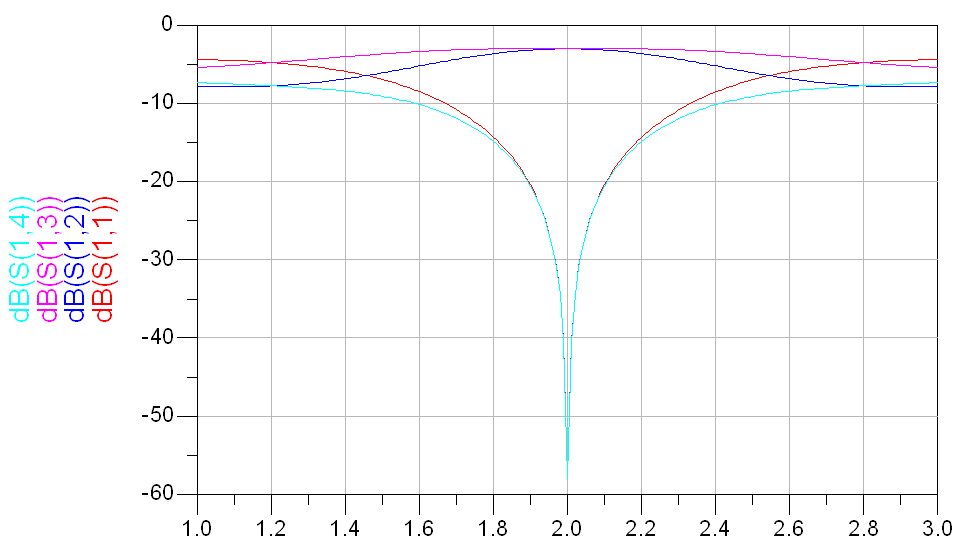
\includegraphics[width=0.5\textwidth]{2.2.png}}
  \subfigure{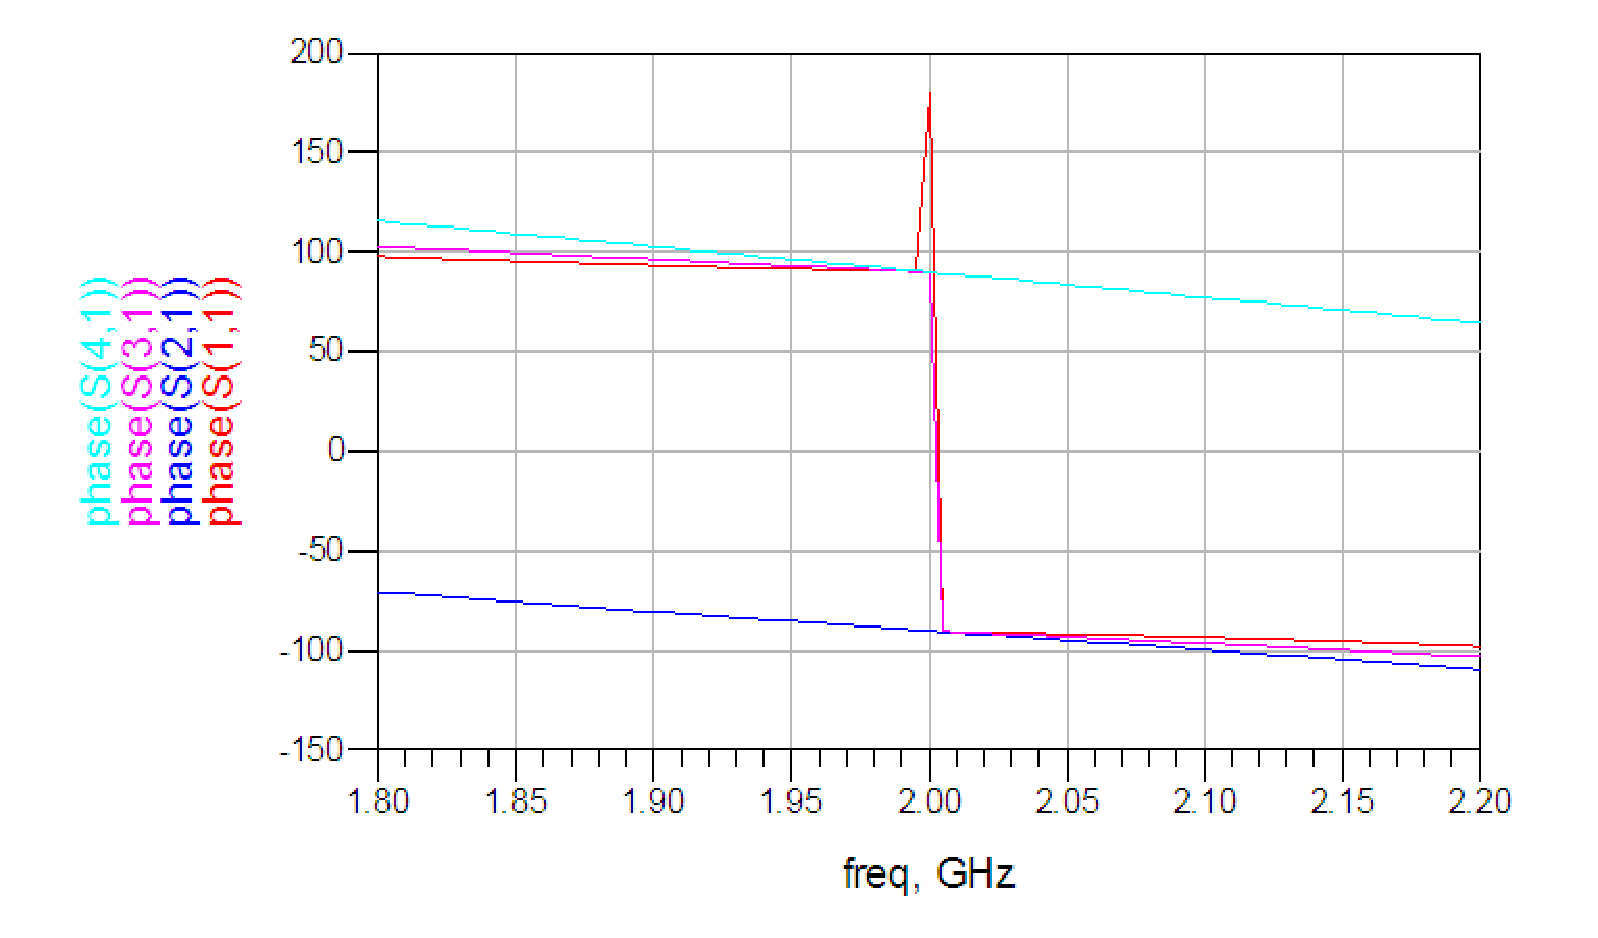
\includegraphics[width=0.5\textwidth]{rat-race-phase.eps}}
  \caption{Magnitude& Phase of S for Rat-Race Coupler}
\end{figure}

\begin{figure}
\centering
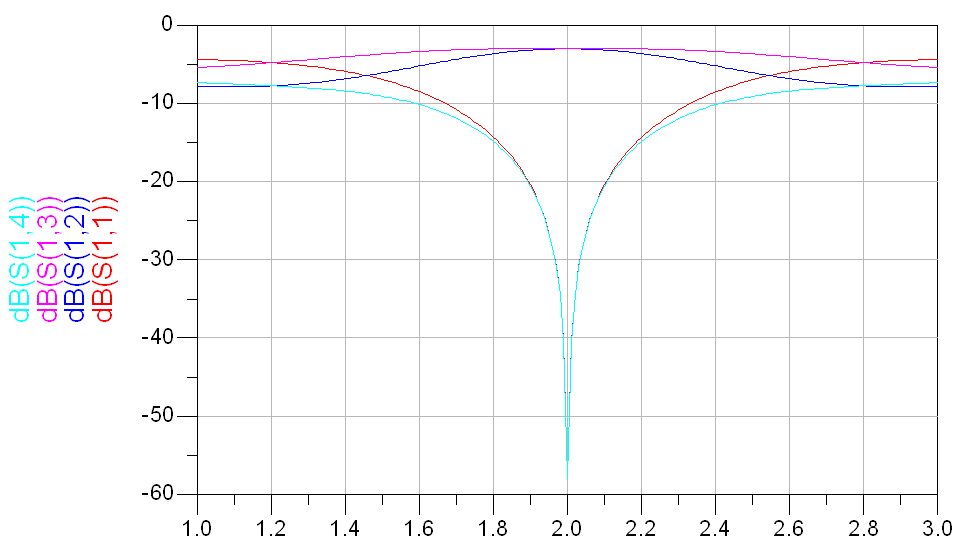
\includegraphics[width=0.5\textwidth]{2.2.png}
\caption{S(1,n) of Rat-Race coupler}
\end{figure}

\begin{figure}
\centering
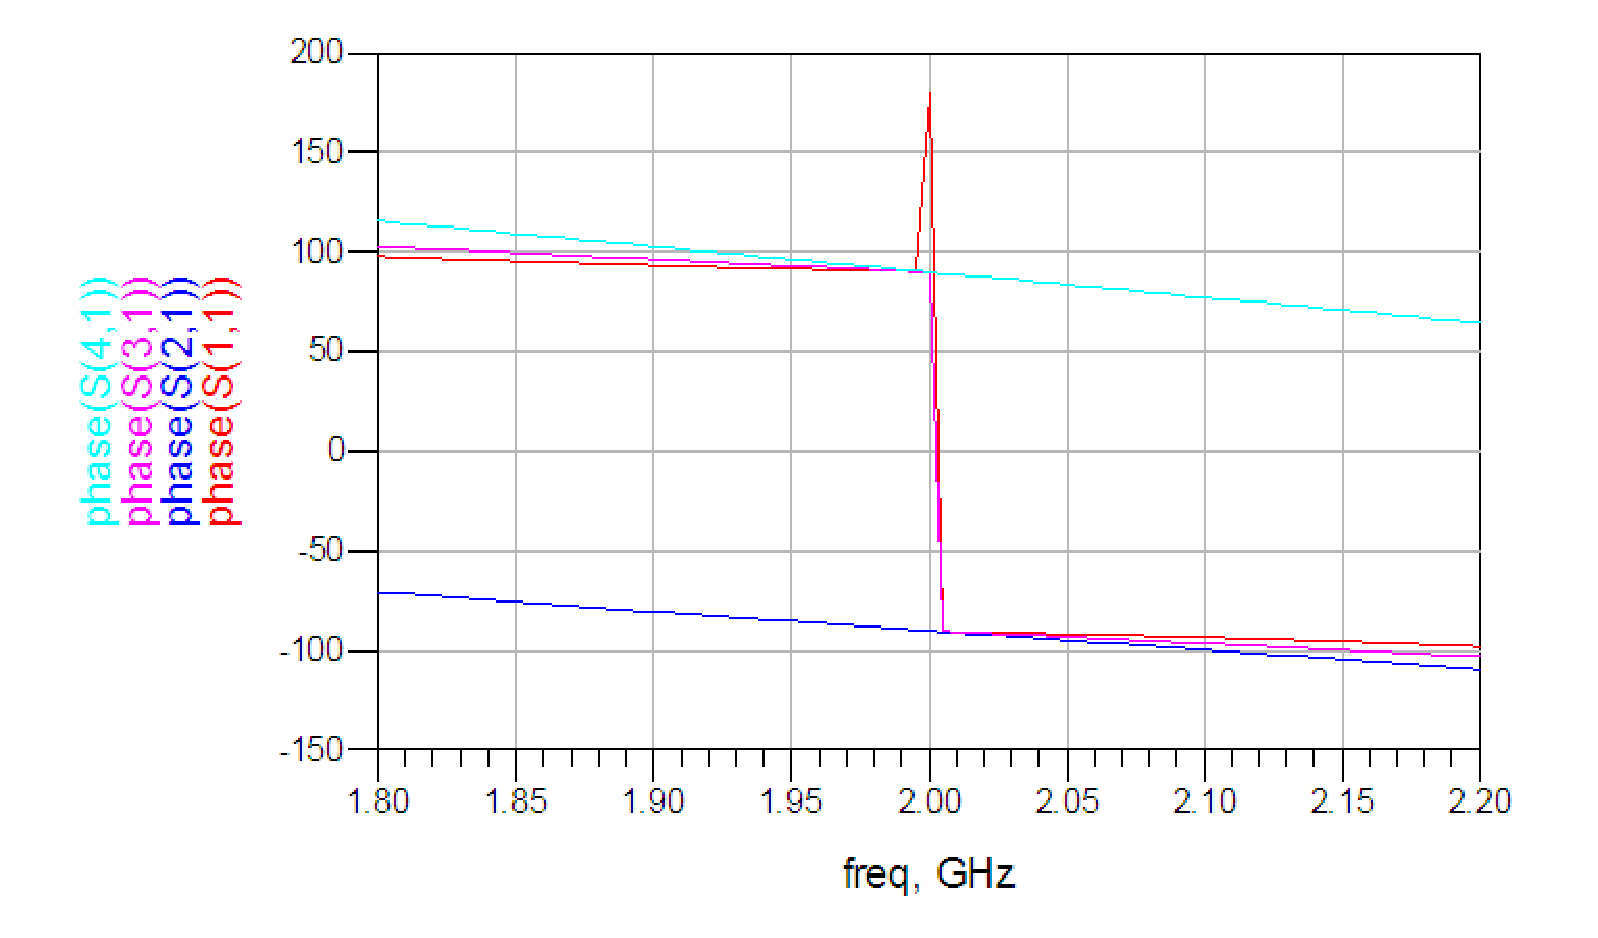
\includegraphics[width=0.5\textwidth]{rat-race-phase.eps}
\caption{phase of Rat-Race coupler}
\end{figure}

\begin{figure}
\centering
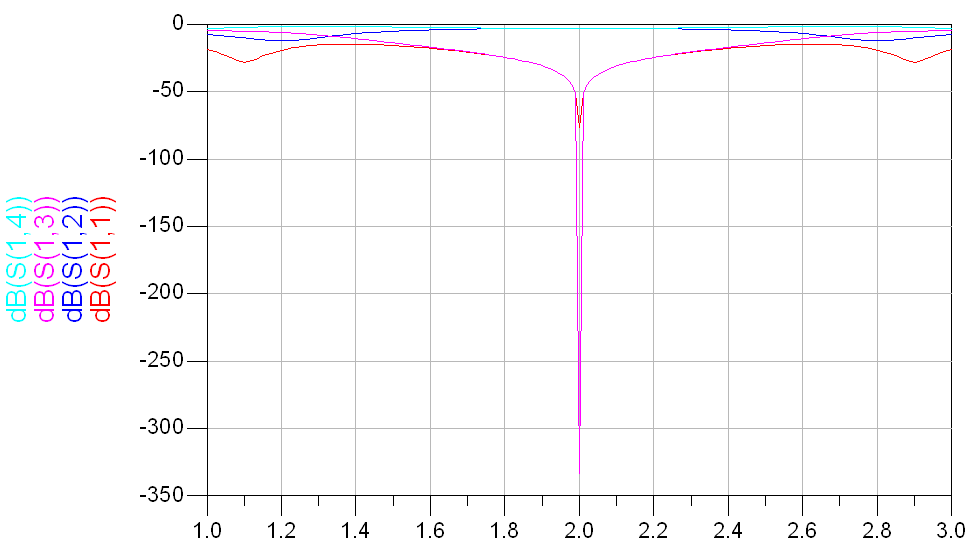
\includegraphics[width=0.5\textwidth]{2.5.png}
\caption{S(1,n) of Branch-Line coupler}
\end{figure}

\begin{figure}
\centering
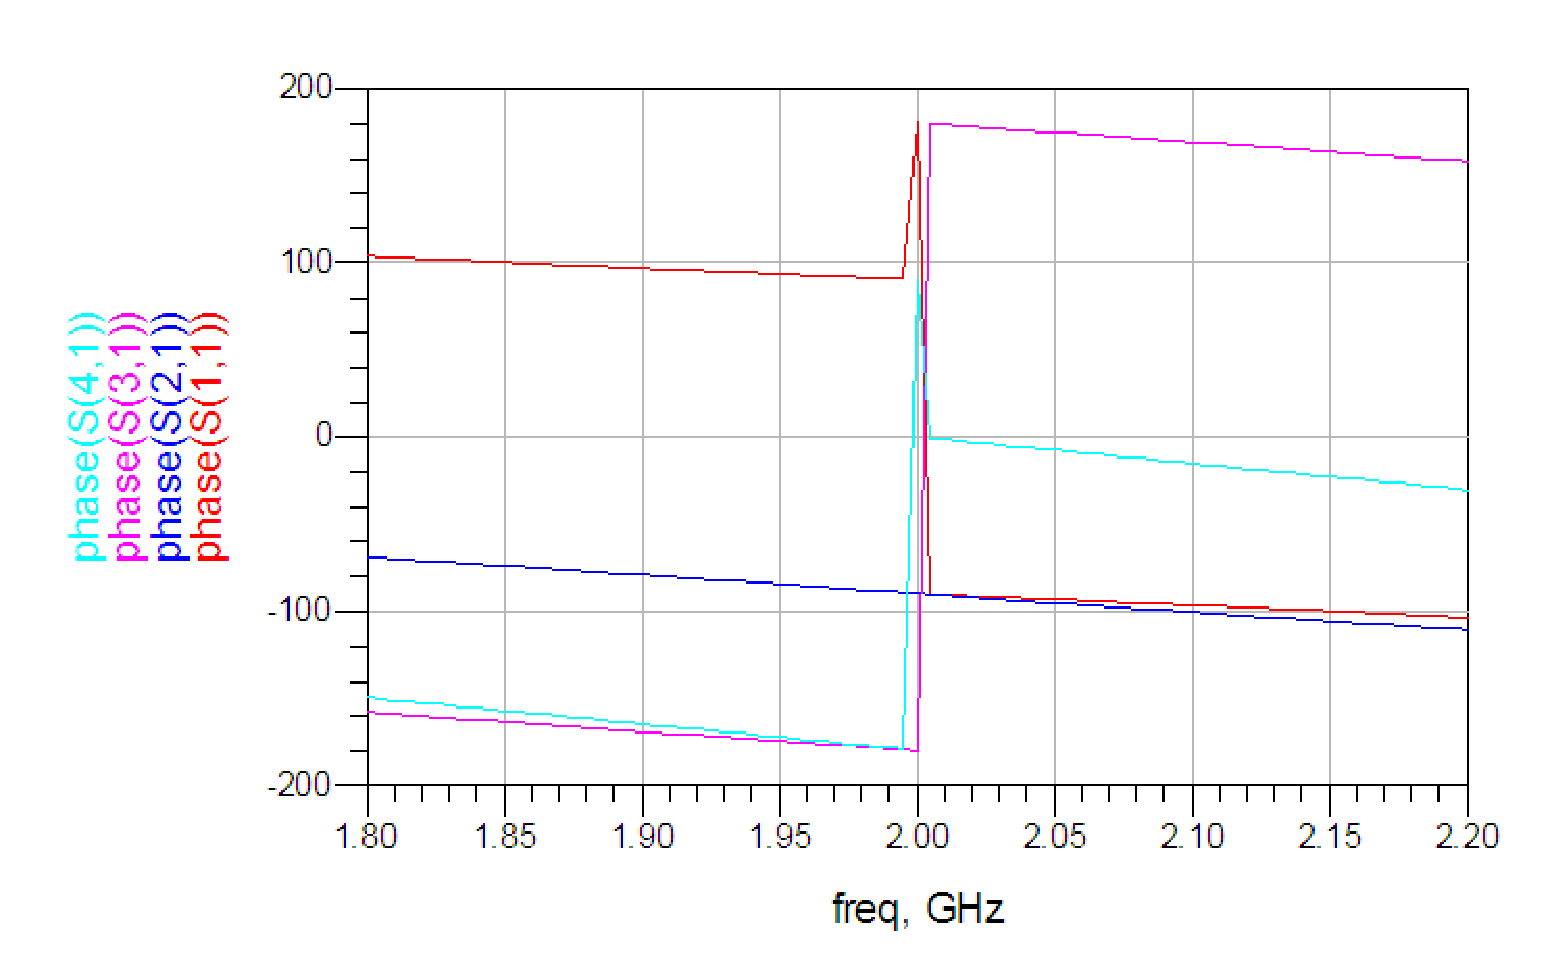
\includegraphics[width=0.5\textwidth]{branch-line-phase.eps}
\caption{phase of Branch-Line coupler}
\end{figure}

\end{document}
